% =====================================================================
%  hc_void_v1.tex  --  Hydrocode sheet, Fig. 3: void (free-surface) ends
%  CARTOON: an empty ghost cell on each side of the mesh, k = 0 on the
%  left and k = k_max + 1 on the right, with M = P = q = 0.  The real
%  boundary faces are 1/2 and k_max + 1/2; their node mass is then half a
%  real cell, which is exactly a free surface (P = 0) for the momentum
%  update.  No numbers.
% =====================================================================
\documentclass[tikz,border=6pt]{standalone}
\usepackage{amsmath,bm}
\usetikzlibrary{arrows.meta,patterns}
\definecolor{slate}{HTML}{2C3E50}
\definecolor{oiblue}{HTML}{0072B2}
\definecolor{oiorange}{HTML}{E69F00}
\begin{document}
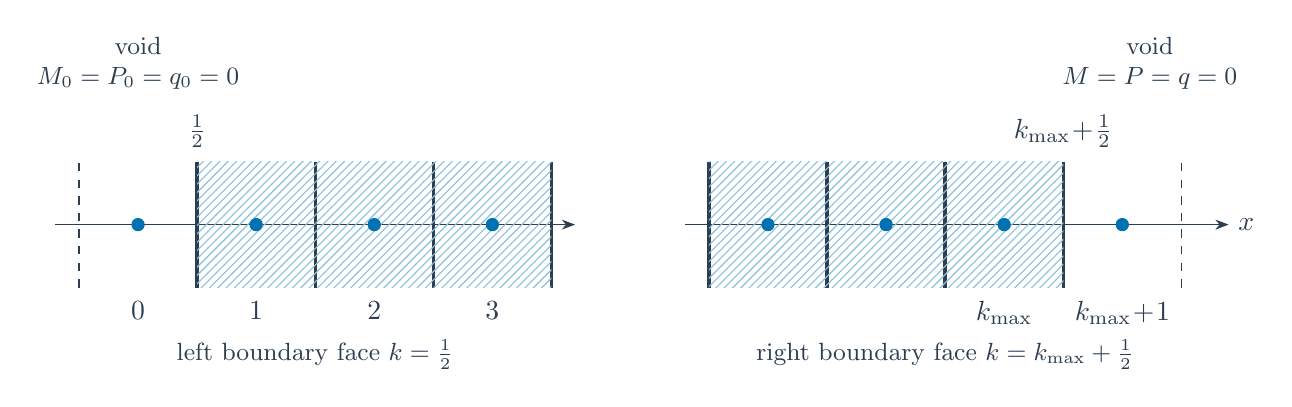
\begin{tikzpicture}[font=\sffamily, text=slate, >=Stealth]
  % LEFT end
  \draw[->,slate,thin] (-0.3,0) -- (6.3,0);
  \draw[slate,dashed] (0,-0.8) -- (0,0.8);
  \foreach \f in {1.5,3.0,4.5,6.0} \draw[slate,line width=1.2pt] (\f,-0.8) -- (\f,0.8);
  \fill[pattern=north east lines, pattern color=oiblue!45] (1.5,-0.8) rectangle (6.0,0.8);
  \foreach \c/\lab in {0.75/0, 2.25/1, 3.75/2, 5.25/3} \fill[oiblue] (\c,0) circle (2.4pt);
  \node[below] at (0.75,-0.85) {$0$};
  \node[below] at (2.25,-0.85) {$1$}; \node[below] at (3.75,-0.85) {$2$}; \node[below] at (5.25,-0.85) {$3$};
  \node[above] at (1.5,0.85) {$\tfrac{1}{2}$};
  \node[align=center,font=\small] at (0.75,2.05) {void\\ $M_0=P_0=q_0=0$};
  \node[font=\small] at (3.0,-1.65) {left boundary face $k=\tfrac{1}{2}$};
  % RIGHT end
  \begin{scope}[xshift=8.0cm]
  \draw[->,slate,thin] (-0.3,0) -- (6.6,0) node[right] {$x$};
  \foreach \f in {0,1.5,3.0,4.5} \draw[slate,line width=1.2pt] (\f,-0.8) -- (\f,0.8);
  \draw[slate,dashed] (6.0,-0.8) -- (6.0,0.8);
  \fill[pattern=north east lines, pattern color=oiblue!45] (0,-0.8) rectangle (4.5,0.8);
  \foreach \c in {0.75,2.25,3.75,5.25} \fill[oiblue] (\c,0) circle (2.4pt);
  \node[below] at (3.75,-0.85) {$k_{\max}$}; \node[below] at (5.25,-0.85) {$k_{\max}\!+\!1$};
  \node[above] at (4.5,0.85) {$k_{\max}\!+\!\tfrac{1}{2}$};
  \node[align=center,font=\small] at (5.6,2.05) {void\\ $M=P=q=0$};
  \node[font=\small] at (3.0,-1.65) {right boundary face $k=k_{\max}+\tfrac{1}{2}$};
  \end{scope}
\end{tikzpicture}
\end{document}
